% -*- root: ../main.tex -*-
%!TEX root = ../main.tex
% this file is called up by main.tex
% content in this file will be fed into the main document
% vim:textwidth=80 fo=cqt

In  order  to establish  a  context  for discussing  the  author's  work, it  is
imperative to provide  a holistic presentation of the  basic \gls{spm} modelling
art. The conventional \gls{spm} is the simplest of all time domain physics-based
models and  the rest  of this  section provides an  expository treatment  of its
rubrics.

\subsection{Geometry}\label{subsec:basicspmgeometry}

\begin{figure}[h]
    \centering
    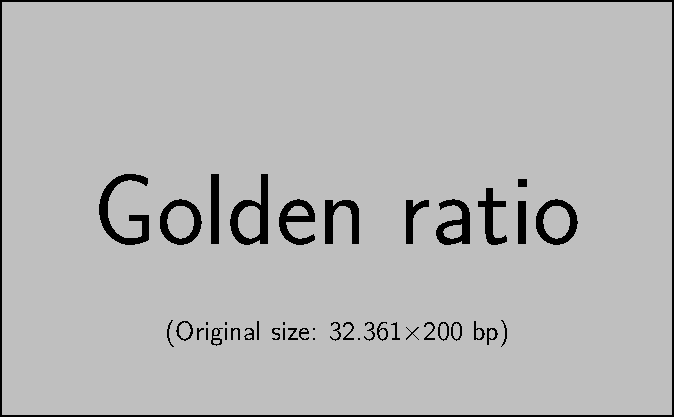
\includegraphics[width=\textwidth]{placeholder_images/example-image-golden.pdf}
    \caption[Schematic illustration depicting geometrical origins of the \gls{spm}]
    {Schematic illustration depicting the geometrical origins of the \gls{spm}.
    The \gls{spm} is obtained through a degenerate spatial discretisation of one
electrochemical layer within a typical Li-ion pouch cell. The axial direction
along the cell's thickness is denoted by $x(t)$, whilst the pseudo-dimension
along the radial depth of each electrode particle is denoted by $r(t)$. In the
basic \gls{spm}, the active material of each porous electrode is represented by
one representative spherical particle, thus entirely eliminating the spatial
dimension along the axial direction.}
    \label{fig:sandwichtospm}
\end{figure}


\Cref{fig:sandwichtospm}  shows the  arrangement  of  one electrochemical  layer
within a  typical Li-ion pouch cell.  A description of the  working principle of
the  cell was  presented in~\cref{ch:chapter1}  and  is not  repeated here.  The
\gls{spm}, as the name suggests,  models the electrochemical phenomena along the
thickness  $l_j$, \jinnegpos{}  of  each porous  electrode  by a  representative
spherical particle.  Thus the two distinct  solid phase porous materials  of the
cell, \ie{} the  negative and positive electrodes, are idealised  as two spheres
of radii $r_\text{neg}$ and $r_\text{pos}$ respectively.


In  this  reformulated  arrangement,  the  spatial  dimension  along  the  axial
thickness  of  each  electrode  degenerates   to  a  single  point.  Hence,  the
concentration of Lithium within each electrode $c_{\text{s}_j}$, \jinnegpos{} is
only a  function of the radial  position $r_j$, \jinnegpos{} along  the depth of
their representative spherical particle, and time, $t$. The surface area of each
representative sphere is scaled appropriately,  such that they are equivalent to
the  active area  of the  corresponding  porous electrodes.  Thus the  \gls{spm}
accounts  for  the  reduced  volume-fraction  arising  due  to  the  microporous
structure of the solid phase. Hence,  the storage capacity of the representative
particles match that of the corresponding electrodes. The overarching assumption
of the \gls{spm} modelling philosophy is that the electrochemical performance of
these representative  electrodes are  sufficient to model  the behaviour  of the
cell at its terminals. The \gls{spm}  thus employs the coarsest possible spatial
discretisation of the cell's thickness with the goal of minimising computational
burden.


\subsection{Scope and Assumptions}\label{subsec:basicspmassumptions}

Having established the geometrical representation of the model, it is imperative
to establish its  aims and scope. This section discusses  the subset of physical
phenomena that can captured by the model and enumerates the inherent assumptions
in  model derivation.The  validity of  these  assumptions and  their effects  is
discussed  in~\cref{subsec:basicspmlimitations}.  As  a  broad  outline  of  the
\gls{spm}s scope,  the model  attributes the cell  polarisation to  two dominant
physics, \viz{}  reaction kinetics  and solid  phase transport  phenomena, \ie{}
diffusion dynamics.


The  \gls{spm}  assumes that  charge  transfer  happens throughout  the  surface
of  each  representative  spherical  particle where  intercalation  occurs.  The
electronic  conductivity of  the solid  phase is  assumed to  be high  enough to
ignore the  spatial distribution of  charge, \ie{} the local  volumetric current
density is assumed  to be uniform along the thickness  of each porous electrode.
This assumption is  motivated by the early calculations performed  by Newman and
Tobias~\cite{Newman1962} in their stand-alone  analysis of current distributions
in porous electrodes, wherein a volume-averaged molar flux is deemed sufficient.
This uniform current density assumption implies that all of the particles in the
electrode active material are in parallel.


In the  \gls{spm}, solid phase  diffusion dynamics  are solved by  assuming this
averaged electrochemical  reaction rate.  In the simulation  study by  Smith and
Wang~\cite{Smith2006b},  it  is  reported  that, soon  after  the  beginning  of
discharge, solid phase concentration and ionic flux become nearly independent of
spatial position, and  Lithium diffusion in solid particles may  be driven by an
averaged molar flux at the surface.


Based  on the  discussion thus  far, it  is clear  that the  \gls{spm} does  not
attempt  to model  all physical  processes within  the cell.  The model  assumes
instantaneous  charge transport  from one  electrode  to the  other through  the
solution phase.  This implies that  electrolytic diffusion is  sufficiently fast
(relative to  diffusion in the solid  phase). Thus, mass transport  phenomena in
the electrolyte are not considered.


During the  operation of the  cell, the  \gls{spm} assumes that  the electrolyte
concentration  $c_\text{e}$ remains  constant at  its equilibrium  initial value
$c_{\text{e},0}$ throughout  the cell thickness. Neglecting  local concentration
gradients  in the  solution phase,  together  with ignoring  its mass  transport
phenomena implies that  the current in the electrolyte does  not vary over space
and time. Hence,  in the conventional \gls{spm} there is  no contribution of the
solution  phase to  internal  overpotentials and  electrolyte  dynamics have  no
influence on the cell's terminal voltage.


Finally,  the  \gls{spm}  ignores  any   variations  in  material  porosity  and
ionic-flow tortuosity  along the axial  direction of the cell.  This facilitates
the  usage of  a constant  effective diffusion  coefficient for  the electrolyte
phase. Furthermore,  all solid  phase diffusivities  and kinetic  parameters are
held constant. Thermal  effects are assumed to be negligible  and no degradation
effects are attempted to be modelled.


These simplifying  assumptions are  made so  as to enable  the formulation  of a
physics-based model without incurring a  heavy computational cost. The impact of
these  assumptions shall  be  examined in~\cref{subsec:basicspmlimitations}  and
later  sections presents  research that  strives  to straddle  the fine  balance
between model sophistication and computational complexity.


\subsection{Chemistry}

This section  provides a  brief overview of  the essential  chemistry principles
that helps to provide a background context for the governing equations presented
in~\cref{subsec:basicspmgoverningeqns}.


In  a Li-ion  cell,  the  positive electrode  consists  of  porous particles  of
Lithium-Transition Metal Oxide (MO)  compounds. The negative electrode typically
employs  some  variant  of  microporous  graphite.  The  porous  nature  of  the
electrodes  provide interstitial  sites  which act  as  intercalation spots  for
Lithium shuttling  between the two  electrodes. The electrolyte,  whose dynamics
are ignored  in the \gls{spm},  helps in the  conduction of \ch{Li^+}  ions. The
separator membrane allows the passage of  these ions between the two electrodes,
but prevents internal short-circuit  by inhibiting electronic conduction through
it. The current collectors facilitate  passage of electrons generated during the
charge transfer reaction  at particle surface to the external  circuit. With the
help of~\cref{fig:chargetransferprocess}  the steps involved in  this process is
detailed next.

\begin{figure}[h]
    \centering
    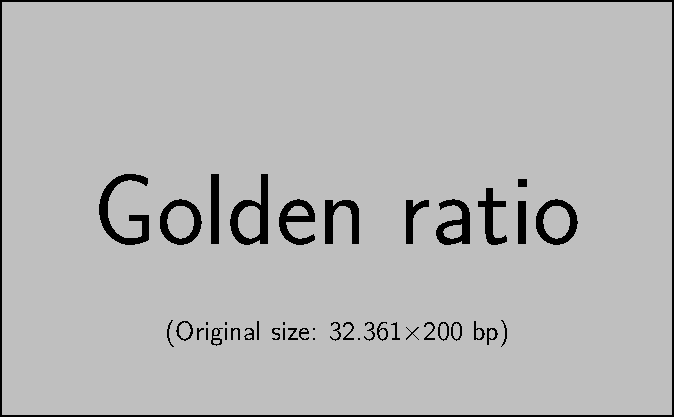
\includegraphics[width=0.5\textwidth]{placeholder_images/example-image-golden.pdf}
    \caption[Charge-transer and basic working mechanism of a Li-ion cell]{Simplified representation of charge-transfer process and illustration of
    basic working mechanism of a Li-ion cell.}
    \label{fig:chargetransferprocess}
\end{figure}

At fully charged  condition, majority of Lithium in the  system is packed within
the negative electrode microstructure. During discharge, \ch{Li^0} atoms diffuse
out  of  deep  interstitial  sites  towards the  surface  of  the  particles  in
the  negative electrode.  At  the surface  (electrode-electrolyte interface),  a
charge-transfer process takes place according to Butler-Volmer kinetics, leading
to  the formation  of \ch{Li^+}  ions and  electrons. The  electrons are  passed
to  the external  circuit  through  \ch{Cu} current  collectors  onto which  the
conductive matrix  composed of  the negative electrode  material and  binders is
coated. The  \ch{Li^+} ions travel  through the electrolyte phase,  crossing the
separator membrane  to the positive  electrode where they encounter  an electron
influx from the external circuit. A  charge transfer reaction takes place at the
surface of the positive electrode particles, leading to the formation of neutral
\ch{Li^0} atoms that diffuse into the positive electrode microstructure.

During  the   charging  process,  the   reverse  phenomena  occur.   Lithium  is
de-intercalated  from  the  positive  electrode and  a  similar  charge-transfer
happens  at the  surface,  leading  to the  formation  of  \ch{Li^+} ions  which
reach  the  negative  electrode  by   passing  through  the  separator.  At  the
surface  of  the  negative  electrode particles,  these  ions  absorb  electrons
from  the  external circuit,  leading  to  the  formation of  neutral  \ch{Li^0}
that   diffuses  into   interior   vacant  spaces   in   the  layered   graphite
electrode. The  charge-transfer mechanism  and sequence  of events  are depicted
in~\cref{fig:chargetransferprocess}.
\Cref{eq:NegElectrodeRxn,eq:PosElectrodeRxn} summarise the reactions during the
charging and discharging process at the surfaces of both electrode materials.
\tikzexternaldisable
\begin{align}
    \ch{Li_{$x$} C                            &<=>[\tiny{discharge}][\tiny{charge}] C + $x$ Li^+ + $x$ e^-}\label{eq:NegElectrodeRxn}\\
    \ch{Li_{1-$x$} M O2 + $x$ Li^+  + $x$ e^- &<=>[\tiny{discharge}][\tiny{charge}] LiMO2}\label{eq:PosElectrodeRxn}
\end{align}
\tikzexternalenable
where    \ch{M}   represents    a    transition   metal    compound   such    as
\ch{Ni_{1/3}Co_{1/3}Mn_{1/3}}   (NMC),   \ch{Ni_{0.8}Co_{0.15}Al_{0.05}}   (NCA)
amongst other  choices~\cite{Reddy2011}. Assuming  no loss of  cycleable Lithium
due to  parasitic side  reactions or  through other  mechanisms, the  process is
fully reversible.


The  electric potential  at  each  electrode is  dependent  upon  the extent  of
its  lithiation. An  empirical  relationship of  each  electrode's potential  as
a  function  of  its  stoichiometry  can be  obtained,  and  is  dependent  upon
the  specific design  and  material  properties of  each  active material  under
consideration. Finally, the \gls{ocv} of the cell is obtained by subtracting the
negative electrode potential from its positive electrode counterpart.

\subsection[Governing  Equations]{Governing  Equations\protect\footnote{In  this
section,   only  those   simplifications  to   mathematical  notations   arising
due  to  assumptions  discussed  in~\cref{subsec:basicspmassumptions}  shall  be
introduced   in-line.   For  a   comprehensive   reference   to  the   notations
used,   please  refer   to   nomenclature   list  in   the~\nameref{ch:glossary}
chapter.  Notations  introduced  solely  for   this  section  are  also  covered
here.}}\label{subsec:basicspmgoverningeqns}


As discussed  in~\cref{subsec:basicspmgeometry}, the \gls{spm}  primarily models
the  cell's dynamics  due to  solid phase  diffusion and  reaction kinetics,  in
addition to embedding the contribution of equilibrium thermodynamics.

\subsubsection*{Solid Phase Diffusion}

Conservation of \ch{Li^0} in the electrodes can be obtained by treating that the
movement of neutral  atoms within the solid phase is  primarily due to diffusion
within particles.  This diffusion  phenomena is induced  due to  a concentration
gradient  that  exists  between  the  surface and  interior/core  of  the  solid
phase  particles. Based  on  the  geometrical assumptions  of  the \gls{spm}  as
discussed in~\cref{subsec:basicspmgeometry}, \ie{} owing  to the lack of spatial
discretisation in the axial direction $x$, the concentration of \ch{Li^0} in the
two electrodes $c_\sj(x,r,t)$,  reduces to a function of  the radial co-ordinate
$r$ and  time $t$,  and is  denoted by $c_\sj(r,t)$,  \jinnegpos{}. To  keep the
notation tractable, this explicit  spatio-temporal radial dependence is omitted,
further simplifying the representation to $c_\sj$.

Diffusion effects  in the solid phase can be modelled  by applying  classical
Fickian dynamics given by
\begin{equation}\label{eq:cartesiandiffusion}
    \diffp{c_\sj}{t} = ∇\! ⋅ \left(D_\sj\, ∇ c_\sj \right)\qquad \jinnegpos{}\footnotemark{}
\end{equation}
\footnotetext{For  the  sake of  brevity,  in  rest  of  the equations  in  this
section,  the  explicit  definition  for   each  subsequent  occurrence  of  the
subscripted variable $j$ shall be omitted. It is implied that \jinnegpos{} since
these  equations describe  solid phase  diffusion in  the negative  and positive
electrodes.}  The divergence  of  a vector  field  $\mathbf{F}(r,θ,ϕ)$ can  be
expressed in spherical co-ordinates as
\begin{equation}\label{eq:fullsphericaldiv}
    ∇ ⋅ \mathbf{F} = \frac{1}{r^2}\diffp{\left(r^2 F_r\right)}{r} +
    \frac{1}{r \sin θ}\diffp{\left(\sin θ\:  F_θ\right)}{θ}
    + \frac{1}{r \sin θ}\diffp{F_ϕ}{ϕ}
\end{equation}
where $r$ denotes the radial magnitude, $θ$ the polar angle and $ϕ$, the
azimuthal angle. $F_r, F_θ$ and $F_ϕ$ denote the corresponding
components of the vector field $\mathbf{F}$.

The centre  of the  co-ordinate system  for each electrode  is aligned  with the
centre of  its representative spherical particle.  Due to symmetry in  the polar
and  azimuthal axes,  the  divergence  becomes a  function  of  only the  radial
position and~\cref{eq:fullsphericaldiv} reduces to
\begin{equation}\label{eq:reducedsphericaldiv}
    ∇ ⋅ \mathbf{F} = \frac{1}{r^2}\diffp{\left(r^2 F_r\right)}{r}
\end{equation}
Applying the divergence operator of~\cref{eq:reducedsphericaldiv}
in~\cref{eq:cartesiandiffusion} yields
\begin{equation}\label{eq:csdiffusioneqn}
    \diffp{c_\sj}{t} = \frac{1}{r^2}\diffp*{\left(r^2 D_\sj\, ∇ c_\sj \right)}{r}
\end{equation}
As   per  the   assumption   of   uniform  diffusivity   in   the  solid   phase
(see~\cref{subsec:basicspmassumptions}),~\cref{eq:csdiffusioneqn} becomes
\begin{align}
    \diffp{c_\sj}{t} &= \frac{D_\sj}{r^2}\diffp*{\left(r^2 ∇ c_\sj \right)}{r}\label{eq:csdiffusionconstdiffusivity}
    \intertext{Applying the gradient operator of~\cref{eq:csdiffusionconstdiffusivity} along
    the radial direction $r$ results in}
    \diffp{c_\sj}{t} &= \frac{D_\sj}{r^2}\diffp*{\left(r^2 \diffp{c_\sj}{r} \right)}{r}\label{eq:csdiffusionfinal}
\end{align}
\Cref{eq:csdiffusionfinal}  represents  the   mass-balance  equation  describing
solid  phase  diffusion in  each  electrode.  The  potential at  each  electrode
depends  on   the  solid  phase  surface   concentration~$c_\sjsurf$  \ie{}  the
\ch{Li^0} concentration $c_\sj(r,t)$ evaluated  at $r=R_\pj$, \jinnegpos{} where
$R_\text{p}$ represents  the equivalent radius of  each representative spherical
particle.  Diffusion in  the solid  phase is  driven by  concentration gradients
induced due  to intercalation  flux density  at the  particle surface,  which is
examined next.

Due to spherical symmetry,  flux at the centre of the  particle is considered to
be zero
\begin{equation}\label{eq:csfluxcentre}
    \diffp{c_\sj}{r}{r=0} = 0
\end{equation}
The   surface  of   each   particle  experiences   a   pore-wall  flux   density
driven  by  reaction  kinetics.  Based   on  the  \gls{spm}  geometry  discussed
in~\cref{subsec:basicspmgeometry}  the spatial  dependence  of  this molar  flux
density  $j_\nj(x,t)$  is  eliminated  and can  be  represented  as  $j_\nj(t)$,
\jinnegpos{}. For the sake of brevity,  the explicit temporal dependence is also
omitted  resulting in  a simplified  notation  $j_\nj$. Hence,  at the  particle
surface
\begin{equation}\label{eq:csfluxsurface}
    D_\sj\diffp{c_\sj}{r}{r=R_\pj} = -j_\nj
\end{equation}
The sign convention chosen here is such that pore-wall flux leaving the particle
surface is considered to be positive.

Charge   conservation   in   solid   phase    is   applied   to   evaluate   the
\gls{rhs}  in~\cref{eq:csfluxsurface},   a  detailed  derivation  of   which  is
presented  in  Domenico~\etal~\cite{DiDomenico2010}.  In  summary,  by  assuming
a  uniform   charge  density   throughout  the   thickness  of   each  electrode
(see~\cref{subsec:basicspmassumptions}),~\cref{eq:csfluxsurface} becomes
\begin{align}
    j_\nj(t)                       &= ± \frac{I(t)}{A \, l_j a_\sj F}\label{eq:uniformcurrdensity}   \qquad \jinnegposordered
    \shortintertext{Substituting~\cref{eq:uniformcurrdensity} in~\cref{eq:csfluxsurface},}
    D_\sj\diffp{c_\sj}{r}{r=R_\pj} &= ∓ \frac{I}{A \, l_j a_\sj F}\label{eq:csfluxsurfacefinal} \qquad \jinnegposordered
\end{align}
wherein   the  load   current  $I(t)   >  0$   for  discharge,   whose  explicit
time-dependence has been  omitted in~\cref{eq:csfluxsurfacefinal} for consistent
notation  with the  \gls{lhs}.  The positive  and negative  signs  apply to  the
negative  and  positive  electrode  respectively as  indicated  by  the  ordered
pair  \jinnegposordered.  In   the  interest  of  completeness,   it  should  be
noted  that  the   term  involving  the  Faraday's  constant   in  the  gls{rhs}
of~\cref{eq:uniformcurrdensity} is  $nF$, where $n$  is the number  of electrons
transferred  during the  reaction.  However, since  this  thesis only  discusses
lithium-ion chemistries  where $n=1$, this  is implicitly conveyed and  shall be
omitted for all possible occurrences.

The \gls{soc} of the cell can be obtained from the bulk concentration of lithium
in either the negative or positive electrode. By convention, negative electrode
is used in computations.
\begin{equation}\label{eq:socinitialdefn}
    z(t) = \frac{3}{c_\snegmax}∫_0^{R_\pneg}r^2 c_\sneg (r,t)\, dr
\end{equation}
Given  an  initial  cell  \gls{soc}  $z(0)  =  z_0$  at  rest,  the  equilibrium
concentration of \ch{Li^0} in the two individual electrodes can be computed as
\begin{equation}\label{eq:csfluxinitialcondition}
    c_\sj(r,0) = c_\sjmax \, \bigg[z_0 \left(θ_\maxj - θ_\minj \right) + θ_\minj \bigg]
\end{equation}

\Cref{eq:csdiffusionfinal},          its         corresponding          boundary
conditions~\eqref{eq:csfluxcentre}  \&~\eqref{eq:csfluxsurfacefinal} along  with
initial   condition~\eqref{eq:csfluxinitialcondition}   provide   the   complete
description   of  time-domain   evolution   of  lithium   in  the   conventional
\gls{spm}   for  a   given  applied   current  profile   $I(t)$.  Considerations
for  efficient   numerical  simulation   of  this   system  is   presented  next
in~\cref{subsec:basicspmgeometry}.


\subsubsection*{Further Reduction in Dimensionality}\label{subsec:basicspmfurtherdimensionalityreduction}

A  naive approach  to numerically  solving  the solid  phase diffusion  equation
is  to  discretise each  of  the  two  representative  particles in  the  radial
direction  as  shown   in~\cref{fig:radialdiscretisation}.  A  three-dimensional
cut-away view  of the division  of the solid  particle into sub-shells  is shown
in~\cref{subfig:radialdisc3d}. Whilst  this schematic conforms to  the \gls{spm}
geometry presented in~\cref{subsec:basicspmgeometry}, it is easier to provide an
annotated illustration using the 2D visualisation of~\cref{subfig:radialdisc2d}.
However, it should  be noted that the actual numerical  computation is performed
using a  one-dimensional mesh, congruent  with the 1D radial  diffusion equation
of~\cref{eq:csdiffusionfinal}.  \Cref{subfig:radialdisc1d}   shows  a  schematic
illustration of this computational domain.
\begin{figure}[h]
    \centering
    \begin{subfigure}[b]{0.3\textwidth}
        \centering
        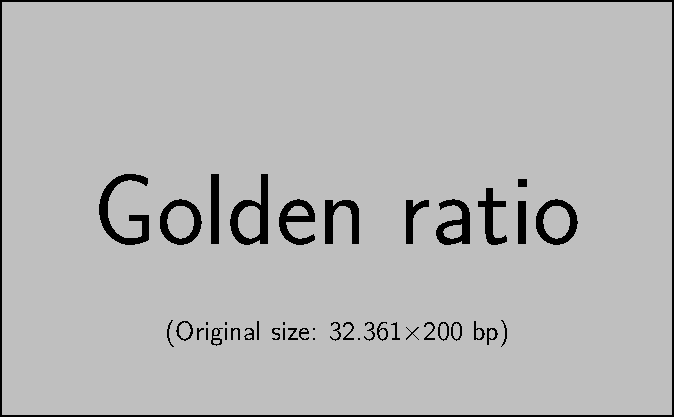
\includegraphics[width=\textwidth]{placeholder_images/example-image-golden.pdf}
        \caption{cutaway view depicting spherical shells}
        \label{subfig:radialdisc3d}
    \end{subfigure}
    \hfill
    \begin{subfigure}[b]{0.3\textwidth}
        \centering
        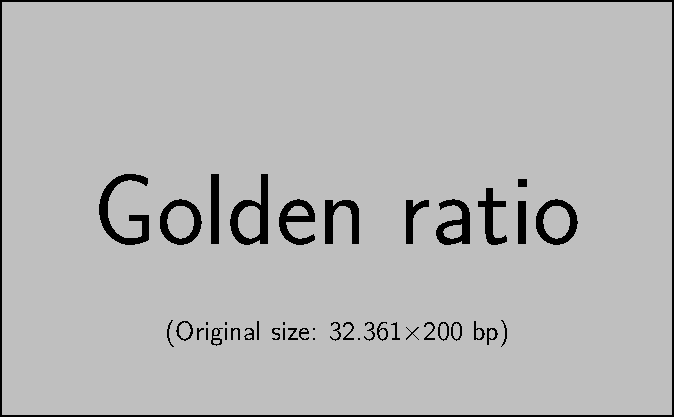
\includegraphics[width=\textwidth]{placeholder_images/example-image-golden.pdf}
        \caption{2D view wherein shells are depicted as concentric rings}
        \label{subfig:radialdisc2d}
    \end{subfigure}
    \hfill
    \begin{subfigure}[b]{0.3\textwidth}
        \centering
        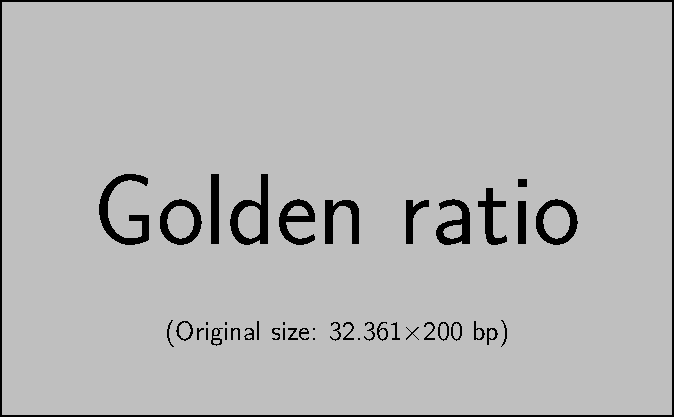
\includegraphics[width=\textwidth]{placeholder_images/example-image-golden.pdf}
        \caption{schematic of 1D computational domain}
        \label{subfig:radialdisc1d}
    \end{subfigure}
    \caption{Radial discretisation scheme for solid phase diffusion.}
    \label{fig:radialdiscretisation}
\end{figure}

Given  the elaborate  simplifications  made to  remove  spatial resolution  from
the  axial  direction,  the  efficacy   of  using  a  radial  discretisation  is
rendered  questionable, particularly  within the  scope of  embedding the  model
in  an  online  simulation  and state-estimation  environment.  Since  diffusion
in  each  spherical  particle  is   modelled  by  well-known  Fickian  dynamics,
several attempts  have been  made to obtain  an approximate  analytical solution
for  the  solid phase  concentration  in  both  electrodes.  In the  context  of
\gls{spm}  modelling,  the  earliest  such  work,  \ie{}  a  comparison  of  the
discretised  version  with  an  approximate analytical  solution  was  performed
by  Santhanagopalan~\etal~\cite{Santhanagopalan2006}.  Zhang and  White  provide
a   comparative  evaluation   of  the   various  approximation   methods  in   a
dimensionless analysis  study~\cite{Zhang2007}, a summary of  which is presented
in~\cref{tbl:solidphaseapprox}.

% -*- root: ../main.tex -*-
%!TEX root = ../main.tex

\begin{table}[h]
    \caption[Solid phase diffusion approximation methods]{Summary of approximation methods for solid phase diffusion}
    \label{tbl:solidphaseapprox}
    \centering
    \begin{tabular}{@{}ll@{}}\toprule
        Method                     & Introduced by                                             \\ \midrule
        Duhamel's superposition    & Doyle, Fuller \&  Newman~\cite{Doyle1993,Fuller1994}      \\
        Diffusion length           & Wang~\etal~\cite{Wang1998}                                \\
        Corrected Diffusion length & Wang and Srinivasan~\cite{Wang2002}                 \\
        Polynomial approximation   & Subramanian~\etal~\cite{Subramanian2001a,Subramanian2005} \\
        Pseudo steady-state        & Liu~\cite{Liu2006}                                        \\
        \bottomrule
    \end{tabular}
\end{table}


The  computational  requirements, \viz{}  storage  and  CPU times  of  Duhamel's
superposition  method  was found  to  be  excessively  high to  warrant  further
interest in it. The original diffusion length method proposed by Wang~\etal{} is
valid  only  after the  diffusion  layer  builds up  to  its  steady state,  and
hence leads  to significant  errors in transient  conditions. Although  Wang and
Srinivasan introduced  an empirical  correction factor  to the  diffusion length
to  extend  its validity  to  short-time  scale  operations, this  affected  the
convergence of the method to the exact solution for steady state conditions. The
pseudo steady  state solution proposed by  Liu uses a finite  integral transform
technique  to eliminate  the  radial dependence  of  solid phase  concentration.
However,   this  method   uses  computations   involving  infinite   summations,
exponential and  trigonometric quantities,  which makes  it less  attractive for
online implementations.

The   literature   on   polynomial  methods   by   Subramanian~\etal{}   provide
detailed derivations  of \engordnumber{2} and  \engordnumber{4}~order polynomial
approximations.  The  \engordnumber{2}~order solution  was  found  to have  poor
performance for transient  behaviour, similar to that of  the original diffusion
length method.  However, higher  order polynomial  approximations were  found to
provide an acceptable  level of performance for both transient  and steady state
conditions and shall be examined further.

The  polynomial   approximation  method  describes  the   dynamic  evolution  of
the  volume  averaged concentration
\begin{equation}
    c_\sjavg(t)  = \frac{1}{Ω}  ∫\limits_Ω c_\sj(r,t)\,  dΩ
\end{equation}
as a function of the applied  load current $I(t)$. Here, $Ω$ represents the
volume  of the  spherical  particle. For  notational  brevity, $c_\sjavg(t)$  is
shortened to $\mean{c}_\sj$ whilst dropping its explicit time dependence.

The \engordnumber{4}~order polynomial approximation assumes that the solid phase
concentration $c_\sj(r,t)$ is a quartic function of the radial co-ordinate $r$
\begin{equation}
    c_\sj(r,t) = a(t) + b(t)\left(\frac{r}{R_\pj}\right)^2 + d(t) \left(\frac{r}{R_\pj}\right)^4
\end{equation}

The     derivation     of     the      coefficients     $a(t),     b(t)$     and
$c(t)$     is     provided    in     Subramanian~\etal{}~\cite{Subramanian2005}.
\Cref{eq:csmeanevolution,eq:qmeanevolution,eq:csurffromcsavg}    summarise   the
governing   equations   obtained    by   applying   the   \engordnumber{4}~order
polynomial        approximation        to         the        system        given
by~\cref{eq:csdiffusionfinal,eq:csfluxcentre,eq:csfluxsurfacefinal}.
\begin{align}
    \diff*{\mean{c}_\sj}{t} + 3\frac{j_\nj}{R_\pj}                                                &=0 \label{eq:csmeanevolution} \\
    \diff*{\mean{q}_j}{t} + 30\frac{D_\sj}{R_\pj^2}\mean{q}_j + \frac{45}{2}\frac{j_\nj}{R_\pj^2} &=0 \label{eq:qmeanevolution}\\
    35\frac{D_\sj}{R_\pj}\left(c_\sjsurf - \mean{c}_\sj\right) - 8D_\sj \mean{q}_j                &= -j_\nj \label{eq:csurffromcsavg}
\end{align}
where $\mean{q}_j(t)$  represents the  volume averaged concentration  flux, that
defines the average change of concentration  with respect to the radial position
$r$.

As   per~\cref{eq:uniformcurrdensity},   the   interfacial   flux   density   is
proportional to  the applied current. Hence~\cref{eq:csmeanevolution}  implies a
simple linear  relationship between the  rate evolution of evolution  of average
\ch{Li^0} concentration within each spherical  particle and the applied current.
This further implies that the \gls{soc} of the cell has a linear rate-dependence
on the externally applied current. Furthermore, due to the elimination of radial
discretisation, the  computation of \gls{soc}  given by~\cref{eq:socinitialdefn}
reduces  to  the   tasks  of  first  computing  the  ratio   of  bulk  (average)
concentration to surface concentration and then  adjusting it to account for the
useable  stoichiometry limits  for that  electrode. Thus,  the \gls{soc}  of the
\gls{spm} can be computed as
\begin{equation}
    z = \frac{\tfrac{\mean{c}_\sneg}{c_\snegmax} - θ_\minneg}{θ_\maxneg - θ_\minneg}
\end{equation}
where $\mean{c}_\sneg$ is obtained by solving~\cref{eq:csmeanevolution} for the
negative electrode.

The \engordnumber{4}~order  polynomial approximation  strikes a  balance between
the three modelling pivots---computational complexity, mathematical tractability
and numerical accuracy, and has been adopted in this work.

At   the   end   of    this   dimension-reduction   step,   spatial   dependence
is   completely  eliminated,   yielding   a  zero-order   (in  space)   physical
model    whose    dynamics   are    described    by    the   \gls{dae}    system
of~\cref{eq:csmeanevolution,eq:qmeanevolution,eq:csurffromcsavg}.

% Thermodynamics, kinetics and state-space formulation  of the model are presented
% next in~\cref{subsec:basicspmthermodynamics}.

\subsubsection*{Equilibrium Thermodynamics}\label{subsec:basicspmthermodynamics}

The equilibrium potential of a porous electrode is a thermodynamic property that
depends on the extent of lithiation in the outermost interstitial sites near the
solid-electrolyte interface.  This surface  stoichiometry $θ_j$ is  obtained by
computing the surface  concentration (see~\cref{eq:csurffromcsavg}) and dividing
by the maximum lithiation capacity of that electrode.
\begin{equation}
    θ_j = \frac{c_\sjsurf}{c_\sjmax}
\end{equation}

Although based upon the theoretical foundation  laid out by the Nernst equation,
owing  to a  multitude of  complex phase  transitions, the  potential of  porous
electrodes  (with respect  to metallic  lithium) is  usually given  as empirical
functions of its surface stoichiometry.
\begin{equation}\label{eq:ocpstoichiometry}
    U_j(t) = \mathcal{U}_j\left(θ_j(t)\right)
\end{equation}
where  the  empirical relationships  $\mathcal{U}_j$  are  typically high  order
polynomials  or rational  functions fitted  to relaxation  data from  \gls{gitt}
experiments on half-cells~\cite{Birkl2015a,Ecker2015}.

In the \gls{spm},  the cell's \gls{ocp} is obtained by  subtracting the negative
electrode  equilibrium  potential  $U_\text{neg}$ from  its  positive  electrode
counterpart $U_\text{pos}$.
\begin{equation}\label{eq:ocpdefinition}
    U_\text{ocp} = U_\text{pos} - U_\text{neg}
\end{equation}
Even though the  concept of \gls{ocp} is defined only  in equilibrium conditions
when no  current flows,  the individual electrode  potentials themselves  form a
significant component of the cell's terminal voltage $V(t)$.

\subsubsection*{Reaction Kinetics}

In the \gls{spm}, the reaction kinetics in each spherical electrode is modelled
using the Butler-Volmer expression
\begin{align}
    j_\nj   &= j_{0_j} \left[ \exp\left( \frac{\left(1-α\right) F η_j}{R T}\right) -  \exp\left( \frac{-α F η_j}{R T}\right)\right] \label{eq:bvwithalpha} \\
    \shortintertext{where}
    j_{0_j} &= k_\jr c_\text{e}^{1-α} c_\sjsurf^{α} \left(c_\sjmax - c_\sjsurf\right)^{1-α}
\end{align}

The  equilibrium rate  of  forward  and backward  reactions  at both  electrodes
is  assumed  to  be  equal.  With   charge  transfer  coefficient  $α  =  0.5$,
\cref{eq:bvwithalpha} simplifies to
\begin{equation}\label{eq:BVwithalphahalf}
    j_\nj = 2 k_\jr \sqrt{c_\text{e} c_\sjsurf \left(c_\sjmax - c_\sjsurf\right)} \sinh\left(\frac{F η_j}{2 R T}\right)
\end{equation}

The    expression    for   overpotential    $η_j$    can    be   obtained    by
rearranging~\cref{eq:BVwithalphahalf}    whilst    substituting   for    $j_\nj$
from~\cref{eq:uniformcurrdensity} and is given by
\begin{equation}\label{eq:overpotential_j}
    η_j(t) =  \frac{2 R T}{F }\sinh^{-1} \left( \frac{± I(t)}{2 A \, l_j a_\sj F k_\jr \sqrt{c_\text{e} c_\sjsurf \left(c_\sjmax - c_\sjsurf\right)}}\right)
\end{equation}

\subsubsection*{Cell Terminal Voltage}\label{subsec:basicspmcellterminalvoltage}

The terminal voltage  of the cell under applied load  is obtained by subtracting
the potential of the negative electrode from its positive counterpart.

Starting from the definition of the overpotential of each electrode
\begin{align}
    η_\text{pos} &= ϕ_\spos - \cancelto{0}{ϕ_\epos} - U_\text{pos} \label{eq:posoverpotential} \\
    η_\text{neg} &= ϕ_\sneg - \cancelto{0}{ϕ_\eneg} - U_\text{neg} \label{eq:negoverpotential}
\end{align}
Within      each      electrode       domain,      the      contribution      of
electrolyte     potential     to      the     overpotential     is     neglected
(see~\cref{subsec:basicspmgeometry,subsec:basicspmassumptions} for  exclusion of
electrolyte dynamics).

Subtracting~\cref{eq:negoverpotential}   from~\cref{eq:posoverpotential}
% whilst substituting for $U_j$ from~\cref{eq:ocpstoichiometry}
\begin{align}
    η_\text{pos} - η_\text{neg} &= \underbrace{ϕ_\spos - ϕ_\sneg}_{V_\text{cell}} - U_\text{pos} + U_\text{neg}\\
\shortintertext{whose rearrangement yields}
    V_\text{cell}               &= η_\text{pos} - η_\text{neg} + U_\text{pos} - U_\text{neg}\label{eq:cellterminalvoltagebasic}
\end{align}
% \mathcal{U}_\text{pos}\left(θ_\text{pos}\right) - \mathcal{U}_\text{neg}\left(θ_\text{neg}\right)
In the  basic \gls{spm},  \cref{eq:cellterminalvoltagebasic} is used  to compute
the   cell's  terminal   voltage  under   load.  Although   the  time-dependence
notation  is  omitted  here,  it   is  worth  reiterating  that  all  quantities
in~\cref{eq:cellterminalvoltagebasic} are functions of time.

\subsubsection*{State Space Representation}\label{subsec:basicspmstatespace}

For control  oriented applications, it is  imperative to have a  classical state
space representation  that collates  all intermediate equations  and definitions
presented  thus  far into  a  single  system  of  equations that  describes  the
evolution of solid concentration and terminal voltage over time as a function of
the  external load  current. However,  the non-linearities  in the  equation for
terminal  voltage  (see~\cref{eq:cellterminalvoltagebasic})  imply  that  it  is
not  possible to  represent  the  \gls{spm} as  the  classical \gls{lti}  system
of~\cref{eq:LTIstatespace}. Instead, the \gls{spm} can be summarised by a system
of linear state equations together with the single non-linear output equation.

The state equation is given by
\begin{equation}\label{eq:fourstatesmatrixvec}
    \setstackgap{L}{1.5\baselineskip}
    \fixTABwidth{T}
    \diff*{\parenMatrixstack{
            \vphantom{\frac{45}{2} \frac{1}{R_\ppos^2 A \, l_\text{pos} a_\spos F}}
            \mean{q}_\text{pos} \\
            \vphantom{\frac{45}{2} \frac{1}{R_\ppos^2 A \, l_\text{pos} a_\spos F}}
            % \vphantom{\frac{D_\sneg}{R_\pneg^2}}
            \mean{q}_\text{neg} \\
            \vphantom{\frac{45}{2} \frac{1}{R_\ppos^2 A \, l_\text{pos} a_\spos F}}
            % \vphantom{\frac{D_\spos}{R_\ppos^2}}
            \mean{c}_\spos \\
            \vphantom{\frac{45}{2} \frac{1}{R_\ppos^2 A \, l_\text{pos} a_\spos F}}
            % \vphantom{\frac{D_\sneg}{R_\pneg^2}}
            \mean{c}_\sneg
        }
    }{t}
    = \underbrace{\parenMatrixstack{
            -30\frac{D_\spos}{R_\ppos^2} & 0                            & 0 & 0 \\
            0                            & -30\frac{D_\sneg}{R_\pneg^2} & 0 & 0 \\
            \vphantom{\frac{45}{2} \frac{1}{R_\ppos^2 A \, l_\text{pos} a_\spos F}}
            0                            & 0                            & 0 & 0 \\
            \vphantom{\frac{45}{2} \frac{1}{R_\ppos^2 A \, l_\text{pos} a_\spos F}}
            0                            & 0                            & 0 & 0
    }}_{A}
    \parenMatrixstack{
        \vphantom{\frac{D_\spos}{R_\ppos^2}}
        \mean{q}_\text{pos} \\
        \vphantom{\frac{D_\sneg}{R_\pneg^2}}
        \mean{q}_\text{neg} \\
        \vphantom{\frac{D_\spos}{R_\ppos^2}}
        \mean{c}_\spos \\
        \vphantom{\frac{D_\sneg}{R_\pneg^2}}
        \mean{c}_\sneg
    }
    +
    \underbrace{\parenMatrixstack{
            \frac{45}{2} \frac{\hphantom{-}1}{R_\ppos^2 A \, l_\text{pos} a_\spos F} \\
            \frac{45}{2} \frac{-1}{R_\pneg^2 A \, l_\text{neg} a_\sneg F} \\
            \hphantom{\frac{45}{2}} \frac{\hphantom{-}3}{R_\ppos  A \, l_\text{pos} a_\spos F} \\
            \hphantom{\frac{45}{2}} \frac{-3}{R_\pneg  A \, l_\text{neg} a_\sneg F}
    }}_{B}
    I(t)
\end{equation}
which corresponds to the classical \gls{lti} form
\begin{equation}
    \dot{\mathbf{x}} = A\,\mathbf{x} + B\,\mathbf{u} \\
\end{equation}
where      $\mathbf{x}     =      \vect{\mean{q}_\text{pos},\mean{q}_\text{neg},
\mean{c}_\spos,  \mean{c}_\sneg},   \,  x   ∈  \mathbb{R}^{4  \times   1}$  is
the  state  vector.  The  scalar   system  input,  $\mathbf{u}  ∈  \mathbb{R}$
is  the  applied  current  $I(t)$.  The  system  matrix,  $A  ∈  \mathbb{R}^{4
\times  4}$  and  input  matrix,  $B ∈  \mathbb{R}^{4  \times  1}$  are  shown
in~\cref{eq:fourstatesmatrixvec}.

For state estimation and controller design purposes, it is important to keep the
number  of elements  in the  state vector  as small  as possible  by eliminating
redundant variables.  Di~Dominico~\etal{}~\cite{DiDomenico2010} noted  that with
output voltage as the only measured quantity, the observablity of the four-state
model of~\cref{eq:fourstatesmatrixvec} is  adversely affected. Consequently, the
following state-reduction approach is proposed.

The total number of moles of lithium in the system is given by
\begin{equation}\label{eq:totallithiummoles}
    n_\text{Li} = \frac{ε_\spos \, l_\text{pos}\, A}{\frac{4}{3} π R_\ppos^3} ∫_0^{R_\ppos} 4 π r^2 c_\spos(r,t) \, dr
    +  \frac{ε_\sneg \, l_\text{neg}\, A}{\frac{4}{3} π R_\pneg^3} ∫_0^{R_\pneg} 4 π r^2 c_\sneg(r,t) \, dr
\end{equation}
Upon considering only the bulk concentration as per the dimensionality reduction
procedure    outlined   in~\cref{subsec:basicspmfurtherdimensionalityreduction},
\cref{eq:totallithiummoles} reduces to
\begin{align}\label{eq:totallithiumsimplified}
    n_\text{Li}  &= \frac{ε_\spos \, l_\text{pos}\, A}{\frac{4}{3} π R_\ppos^3}\mean{c}_\spos ∫_0^{R_\ppos} 4 π r^2  \, dr
    + \frac{ε_\sneg \, l_\text{neg}\, A}{\frac{4}{3} π R_\pneg^3}\mean{c}_\sneg ∫_0^{R_\pneg} 4 π r^2  \, dr
                \\
                 &= ε_\spos \, l_\text{pos}\, A \, \mean{c}_\spos + ε_\sneg \, l_\text{neg}\, A \, \mean{c}_\sneg
\end{align}
Assuming  no  loss  of  cycleable   lithium  or  other  degradation  mechanisms,
the  total   number  of   moles  of   lithium  in   the  system   is  conserved,
\ie{}    $\diff{n_\text{Li}}{t}    =    0$.    Substituting    this    condition
in~\cref{eq:totallithiumsimplified}
\begin{align}
    0                          &= \phantom{+} \diff*{ε_\spos \, l_\text{pos}\, A \, \mean{c}_\spos }{t} + \diff*{ε_\sneg \, l_\text{neg}\, A \, \mean{c}_\sneg }{t} \\
    \diff*{\mean{c}_\spos}{t}  &= -\diff*{\mean{c}_\spos}{t} \label{eq:bulkconcrelationship}
\end{align}

As   per~\cref{eq:bulkconcrelationship},  the   time  evolution   of  the   bulk
concentration  of one  electrode can  be obtained  as a  function of  the other.
Furthermore, Di~Domenico~\etal{}  show that the  diffusion dynamics of  the bulk
concentrations can be algebraically related through their stoichiometric factors
as
\begin{equation}\label{eq:csposbulkfromcsnegbulk}
    \mean{c}_\spos(t) = c_\sposmax \, \bigg[\frac{\mean{c}_\sneg(t)- θ_\minneg
    c_\snegmax}{\left(θ_\maxneg - θ_\minneg\right)c_\snegmax} \left(θ_\maxpos - θ_\minpos \right) + θ_\minpos \bigg]
\end{equation}

Hence,  it is  possible to  eliminate the  bulk concentration  of either  of the
electrodes  from  the state-equation  to  arrive  at a  three-state  description
of  the  model  dynamics.  In   extant  lithium-ion  chemistries,  the  negative
electrode is  considered to  be the  limiting electrode and  is hence  is chosen
here~\cite{Arora1999}. Thus, it is retained in the state vector, thereby leading
to the final form of the state dynamics of the conventional \gls{spm}
\begin{equation}\label{eq:threestatesmatrixvec}
    \setstackgap{L}{1.5\baselineskip}
    \fixTABwidth{T}
    \diff*{\parenMatrixstack{
            \vphantom{\frac{45}{2} \frac{1}{R_\ppos^2 A \, l_\text{pos} a_\spos F}}
            \mean{q}_\text{pos} \\
            \vphantom{\frac{45}{2} \frac{1}{R_\ppos^2 A \, l_\text{pos} a_\spos F}}
            \mean{q}_\text{neg} \\
            \vphantom{\frac{45}{2} \frac{1}{R_\ppos^2 A \, l_\text{pos} a_\spos F}}
            \mean{c}_\sneg
        }
    }{t}
    = \underbrace{\parenMatrixstack{
            -30\frac{D_\spos}{R_\ppos^2} & 0                            & 0  \\
            0                            & -30\frac{D_\sneg}{R_\pneg^2} & 0  \\
            \vphantom{\frac{45}{2} \frac{1}{R_\ppos^2 A \, l_\text{pos} a_\spos F}}
            0                            & 0                            & 0
    }}_{A}
    \parenMatrixstack{
        \vphantom{\frac{D_\spos}{R_\ppos^2}}
        \mean{q}_\text{pos} \\
        \vphantom{\frac{D_\sneg}{R_\pneg^2}}
        \mean{q}_\text{neg} \\
        \vphantom{\frac{D_\spos}{R_\ppos^2}}
        \mean{c}_\sneg
    }
    +
    \underbrace{\parenMatrixstack{
            \frac{45}{2} \frac{\hphantom{-}1}{R_\ppos^2 A \, l_\text{pos} a_\spos F} \\
            \frac{45}{2} \frac{-1}{R_\pneg^2 A \, l_\text{neg} a_\sneg F} \\
            \hphantom{\frac{45}{2}} \frac{-3}{R_\pneg  A \, l_\text{neg} a_\sneg F}
    }}_{B}
    I(t)
\end{equation}

The measured variable $y ∈ \mathbb{R}$ is the cell's terminal voltage
$V(t)$ and is expressed as a non-linear  scalar function of the state vector and
the load current.
\begin{equation}\label{eq:spmoutputeqn}
    y = h(\mathbf{x},u)
\end{equation}
The output  equation given by~\cref{eq:spmoutputeqn} includes  a non-zero direct
feedthrough dependency  of the voltage  on the input current,  thereby modelling
the resistive component of the cell's  impedance. The full expression for output
voltage is given by
\begin{multline}
    V_\text{cell}(t) = \frac{2 R T}{F }\sinh^{-1} \left( \frac{- I(t)}{2 A
    l_\text{pos} a_\spos F k_\posr \sqrt{c_\text{e} c_\spossurf(t)
    \left(c_\sposmax - c_\spossurf(t)\right)}}\right) \\
    - \frac{2 R T}{F }\sinh^{-1} \left( \frac{I(t)}{2 A \, l_\text{neg} a_\sneg F
    k_\negr \sqrt{c_\text{e} c_\snegsurf(t) \left(c_\snegmax - c_\snegsurf(t)\right)}}\right) \\
    + \mathcal{U}_\text{pos}\left(c_\spossurf(t)\right) -
    \mathcal{U}_\text{neg}\left(c_\snegsurf(t)\right)\label{eq:spmbasicoutputvoltagefinal}
\end{multline}
wherein  the solid  phase surface  concentration at  each electrode  $c_\sjsurf$
is   obtained  from   its   corresponding  bulk   concentration  $c_\sjavg$   by
rearranging~\cref{eq:csurffromcsavg} and is given by
\begin{align}
    c_\spossurf &= \mean{c}_\spos  + \frac{8R_\ppos}{35} \mean{q}_\text{pos}
    +\frac{R_\ppos}{35 D_\spos A \, l_\text{pos} a_\spos F} I(t)
    \label{eq:csurfposfromcavgpos}\\
    c_\snegsurf &= \mean{c}_\sneg  + \frac{8R_\pneg}{35} \mean{q}_\text{neg} -\frac{R_\pneg}{35 D_\sneg A \, l_\text{neg} a_\sneg F} I(t)\label{eq:csurfnegfromcavgneg}
\end{align}
where $I(t) > 0 $ for discharge.

Given   the  initial   \gls{soc}  of   the   cell  $z(0)$,   the  initial   bulk
concentration  of   the  negative  electrode  at   equilibrium  $c_\sneg(0)$  is
obtained  by~\cref{eq:csfluxinitialcondition}. The  initial  value  of the  mean
radial  concentration  flux   in  both  electrodes  $q_j(0)   =  0$.  Therefore,
the  initial  state  vector  is $\vect{0,0,c_\sneg(0)}$.  Thus,  the  system  of
equations~\crefrange{eq:csposbulkfromcsnegbulk}{eq:csurfnegfromcavgneg}  form  a
state-space representation of the conventional \gls{spm}. This state-space model
can be simulated as an \gls{ivp} or  used as the plant model in control-oriented
applications such as for dynamic state estimation.
